\documentclass[12pt]{article}

\usepackage{graphicx}
\usepackage{paralist}
\usepackage{amsfonts}
\usepackage{amsmath}
\usepackage{hhline}
\usepackage{booktabs}
\usepackage{multirow}
\usepackage{multicol}
\usepackage{url}

\oddsidemargin -10mm
\evensidemargin -10mm
\textwidth 160mm
\textheight 200mm
\renewcommand\baselinestretch{1.0}

\pagestyle {plain}
\pagenumbering{arabic}

\newcounter{stepnum}

%% Commentshttps://www.overleaf.com/project/606cdf71dae3e549f8784f45

\usepackage{color}

\newif\ifcomments\commentstrue

\ifcomments
\newcommand{\authornote}[3]{\textcolor{#1}{[#3 ---#2]}}
\newcommand{\todo}[1]{\textcolor{red}{[TODO: #1]}}
\else
\newcommand{\authornote}[3]{}
\newcommand{\todo}[1]{}
\fi

\newcommand{\wss}[1]{\authornote{blue}{SS}{#1}}

\title{2048: Design Specification}
\author{Jishan Sharif}

\begin{document}

\maketitle
This Module Interface Specification (MIS) document contains modules, types and
methods for implementing the game \textit{2048}. The rules of the game are as follows. 
The game starts off with a $4x4$ board with two randomly generated values placed in any part of the board. The board is initially empty. The randomly generated values will either be a $2$ or a $4$. We can move either left, right, up or down and for each movement the numbered tile will move to the direction specified. Tiles with the same number merge into one when they touch. Add them up to reach 2048! The game can be launched and played by typing \texttt{make demo} in the terminal.


\begin{center}
  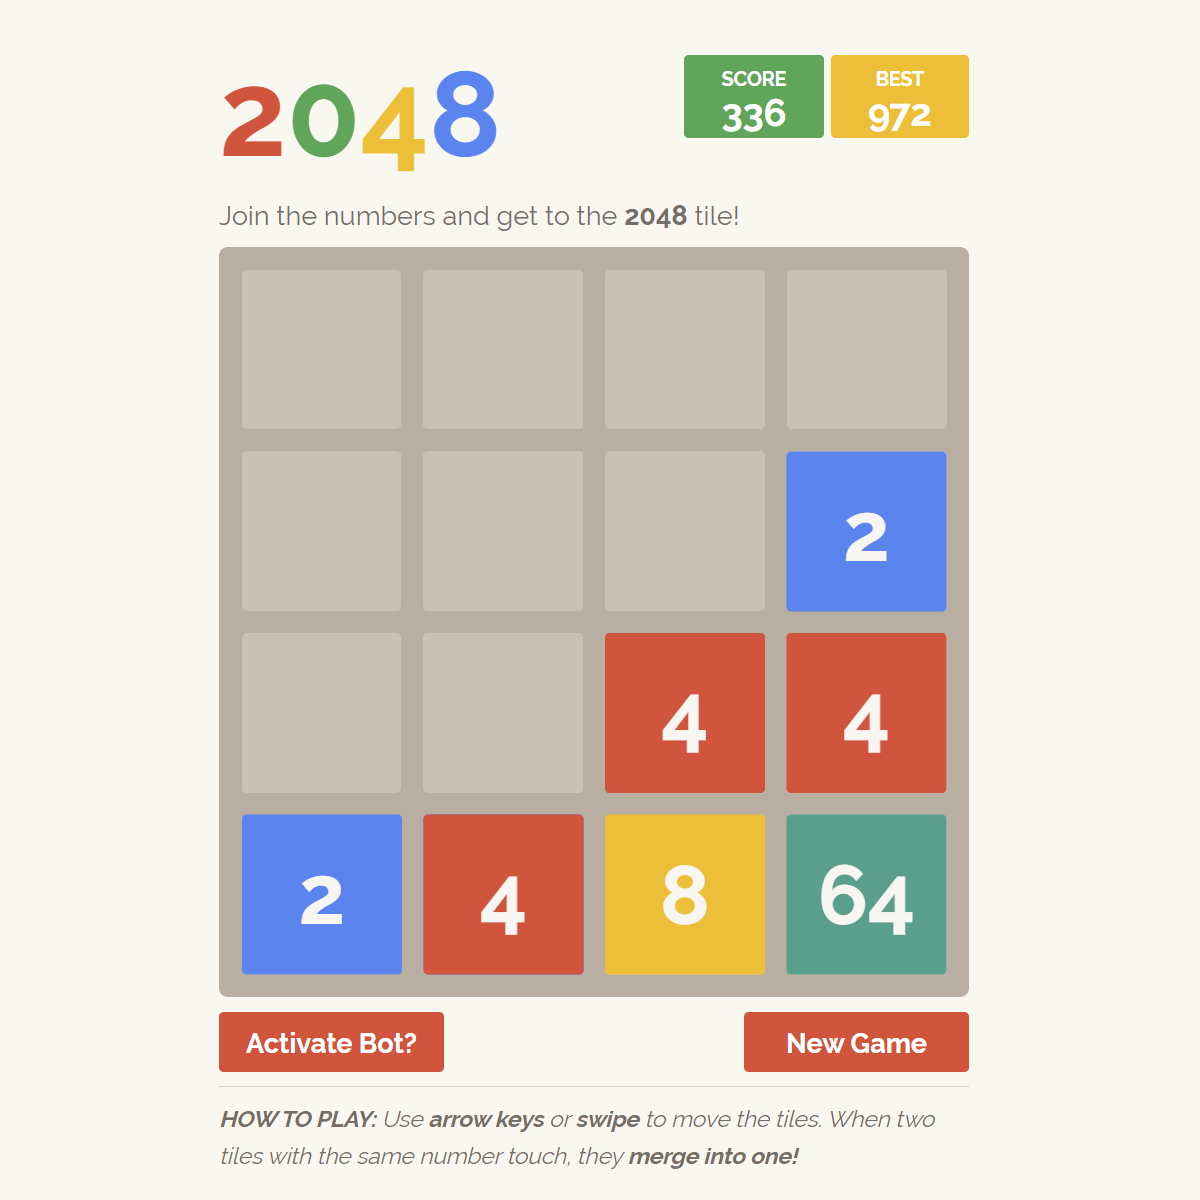
\includegraphics[width=0.7\textwidth]{2048-game.png}

  The above board visualization is from https://elgoog.im/2048/
\end{center}

\newpage

\section{Overview of the design}

Our first step was to initialize the board. The key thing to note about this game is
that we start the game with two randomly placed tiles on a 4x4 board. The score is set to 0.
The filled tiles can have values 2 or 4. It'd be best to create a new Object for a Tile in case we may want to optimize our game to work for different values.

Once we get the board initialized, The next steps was to get the movements to work. There
are four movements to consider on our model, each of these movements can be trigerred using the Controller or the View module

For each movement, I've worked on it using the process of incrementality. The more I worked on each movement, the better I understood the game and the cases required. For the most part,
each movement required precise understanding of board positions and when merging is possible. Furthermore, once this is complete - A point to consider is to check when the game is over. Since a game check would take a longer run time, it's best to make this check after one move is over. Hence, it was most appropriate to add this method onto our controller file.

The difference between this game I've created versus the one available to play online is that empty tiles are denoted as tiles containing the value 0. Any tile which does not contain 0 is a filled tile. In a real game, An empty tile would be a void space.

\subsection*{Likely Changes my design considers:}

The next step would be to wire the game built to a GUI. This would mean refactoring the way the board looks by adding graphics and colours. The most important feature would be to remove the $0$ tiles and add an empty tile. We can also add a points section above the board which updates the points as the game progresses. Currently, we can only view the points by entering the command $p$ on our terminal.

The next thing we could do is make use of a Key Listener instead of asking a User for inputs. This would mean we can make use of arrow keys instead of letters such as $r, l, u, d$ to play the game.

Although this is beyond the scope of this project, it would be ideal to have a previous score saved. This can be the $High Score$ and anytime you beat that, a message can be displayed saying you have beaten the highest score, regardless of the fact whether you won the game or not. We can then update the value of the high score as required.

\newpage

\section* {Tile Type Module}

\subsection*{Module}

TileT

\subsection* {Uses}

N/A

\subsection* {Syntax}

\subsubsection* {Exported Constants}

None

\subsubsection* {Exported Types}

None

\medskip

\noindent \textit{A Board will contain tiles, Each Tile can either be empty or it will contain and integer value.}

\subsubsection* {Exported Access Programs}

\begin{tabular}{| l | l | l | p{6cm} |}
\hline
\textbf{Routine name} & \textbf{In} & \textbf{Out} & \textbf{Exceptions}\\
\hline
TileT & $\mathbb{N}$ & ~ & \\
\hline
setValue & $\mathbb{N}$ & ~ & \\
\hline
getValue & ~ & $\mathbb{N}$ & \\
\hline
toString & ~ & String & \\
\hline
\end{tabular}

\subsection* {Semantics}

\subsubsection* {State Variables}

value: $\mathbb{N}$
\noindent \textit{This value will be initially set to 0}

\subsubsection* {State Invariant}

None

\subsubsection* {Access Routine Semantics}

setValue($\textbf{N}$ $newValue$):
\begin{itemize}
  \item $value= newValue$
\end{itemize}

\noindent getValue():
\begin{itemize}
  \item $out := value$
\end{itemize}

\noindent toString():
\begin{itemize}
  \item $out := intToString(value)$
\end{itemize}

\newpage

\section* {Board ADT Module}

\subsection*{Template Module}

BoardT

\subsection* {Uses}

TileT

\subsection* {Syntax}

\subsubsection* {Exported Types}

None

\subsubsection* {Exported Constant}

Size = 4 \quad // Size of the board 4 x 4

\subsubsection* {Exported Access Programs}

\begin{tabular}{| l | l | l | l |}
\hline
\textbf{Routine name} & \textbf{In} & \textbf{Out} & \textbf{Exceptions}\\
\hline
BoardT & ~ & BoardT & \\
\hline
getScore & ~ & $\mathbb{N}$ & \\
\hline
getBoard & ~ & seq of seq of TileT & \\
\hline
setBoard & seq of seq of TileT & ~ & \\
\hline
moveRight & ~ & ~ & \\
\hline
moveLeft & ~ & ~ & \\
\hline
moveUp & ~ & ~ & \\
\hline
moveDown & ~ & ~ & \\
\hline
noMoreMoves & seq of seq of TileT & $\mathbb{B}$ & \\
\hline
Transpose & ~ & ~ & \\

\hline
\end{tabular}

\subsection* {Semantics}

\subsubsection* {State Variables}

board: sequence [Size, Size] of TileT \\
score: $\mathbb{N}$ \\
moves: $\mathbb{N}$

\subsubsection* {State Invariant}

\noindent \textit{We need to make sure the number of occupied tiles and the number of unoccupied tiles
should be equal to the area of the board}



This is already dealt with when we initialize a 2-D array in Java using the $[][] TileT board = new TileT[size][size]$

\subsubsection* {Assumptions}

\begin{itemize}
  \item The constructor BoardT is called for each object instance before any other access routine
  is called for that object.
  \item Assume there is a random function that generates a random value between 0 and 1.
  \item The board will be initialized with two random values.
\end{itemize}

\subsubsection* {Design decision}

Before we start off, we need to answer a few questions to better construct the game. What would be the best way to represent the board? We are trying to replicate a Matrix so a 2-D ArrayList would work in our example. What will each element contain in the 2-D Matrix, we know the only possible values are either Integers or the element is empty.

What functions do we need for this Board Module and what are the access programs?
We need to verify if any move is considered valid. For every move, we need to update the board. The board will also need a constructor. We would also like to know the state of a certain cell at the game board. This will help us identify if a move is valid or not.
A move is considered invalid when the direction you want the tile to move to cannot move
further. No further merge can take place and the board cannot move in any position. For every merge, a new tile will be placed in any free space at the board. The position of the new tile will once again be randomly generated. Therefore, we know the game will be over when no new tiles cannot be placed, there are no possible merges for any position and the tiles can no longer move. Therefore, we need to know if there are any valid moves left.

Four separate movement functions needs to be made, for each of them, we need to figure out if a merge is possible, if it is, we go ahead and merge them. Mathematics of Matrices tells us that moving up in a matrix is the same as transposing a matrix, moving left and transposing again. This means that our $moveUp$ and $moveDown$ functions will solely depend of the correctness of our $moveLeft$ and $moveRight$ functions accordingly. We will also then need to create a $Transpose$ function which takes in a board and returns the transpose of that board. A transposed board is simply a board with its rows and columns swapped.


\subsubsection* {Access Routine Semantics}

BoardT():
\begin{itemize}
\item transition: \\
      board $:=$
      $\langle \begin{array}{c}
      \langle TileT_0, ... ... ,TileT_3 \rangle\\
      \langle TileT_0, ... ... ,TileT_3 \rangle\\
      \langle TileT_0, ... ... ,TileT_3 \rangle\\
      \langle TileT_0, ... ... ,TileT_3 \rangle\\\
      \end{array} \rangle$ \\
      status, moves $=$ true, 0

      generateValues(board)
\item output: $out := \mathit{self}$
\item exception: None
\end{itemize}

\noindent getScore():
\begin{itemize}
\item transition: none
\item output: $out :=$ score
\item exception: None
\end{itemize}

\noindent getBoard():
\begin{itemize}
\item transition: none
\item output: $out :=$ (board)
\item exception: None
\end{itemize}

\noindent setBoard(newBoard):
\begin{itemize}
\item transition: board = newBoard
\item output: none
\item exception: None
\end{itemize}

\noindent moveRight():
\begin{itemize}
\item transition: None
\item exception: None
\end{itemize}

\noindent moveLeft():
\begin{itemize}
\item output:
\item exception:
\end{itemize}

\noindent moveDown():
\begin{itemize}
\item output:
\item exception:
\end{itemize}

\noindent moveUp():
\begin{itemize}
\item output:
\item exception:
\end{itemize}

\noindent noMoreMoves(board):
\begin{itemize}
\item output:
\item exception:
\end{itemize}

\noindent Transpose():
\begin{itemize}
\item output:
\item exception:
\end{itemize}

\subsubsection* {Local Functions}

\noindent generateValues(board):
\begin{itemize}
\item output:
\item exception:
\end{itemize}


\noindent insertRandom(board):
\begin{itemize}
\item output:
\item exception:
\end{itemize}


\noindent canMergeLeft(i):
\begin{itemize}
\item output:
\item exception:
\end{itemize}


\noindent canMergeRight(i):
\begin{itemize}
\item output:
\item exception:
\end{itemize}

\noindent findEmptyLeftPosition(i):
\begin{itemize}
\item output:
\item exception:
\end{itemize}

\noindent findEmptyRightPosition(i):
\begin{itemize}
\item output:
\item exception:
\end{itemize}

\noindent canMergeTiles(board):
\begin{itemize}
\item output:
\item exception:
\end{itemize}

\noindent isValid(moves):
\begin{itemize}
\item output:
\item exception:
\end{itemize}



\newpage

\section* {View Module}

\subsection* {Uses}

None

\subsection* {Syntax}

\subsubsection* {Exported Types}

None

\subsubsection* {Exported Constants}

None

\subsubsection* {Exported Access Programs}

\begin{tabular}{| l | l | l | p{6cm} |}
\hline
\textbf{Routine name} & \textbf{In} & \textbf{Out} & \textbf{Exceptions}\\
\hline
main & ~ & &  \\
\hline
\end{tabular}

\subsection* {Semantics}


\subsubsection* {State Variables}

greetings\\
start\\
instructions\\

\subsubsection* {State Invariant}

None

\subsubsection* {Assumptions}

\begin{itemize}
\item We assume that the makefile is already set up and we just need to run $make demo$ for the game to work
\end{itemize}

\subsubsection* {Access Routine Semantics}

\noindent main():
\begin{itemize}
  \item print the instructions
  \item print the greetings message
  \item print the board
  \item print the commands available to use
  \item Allow the scanner to use inputs from the reader
  \item Print the state of the game, and whether the game has ended
\end{itemize}

\subsubsection*{Local Function:}

\noindent checkWinner(score):
\begin{itemize}
  \item If the score is below 2048, we return false, else we return true
\end{itemize}

\newpage

\section*{Critique of Design}

\begin{itemize}
  \item I choose to specify BoardT module as ADT over abstract object, because It is more convenient to create a new instance of the board after the
        user choose to restart a game.
  \item The controller and the view is in the same file since it would be easier to control
  the state of the game during runtime.
  \item I returned the points of the game after I enter a specific command, this is not a good idea since the ideal situation would want to know their points after each move. They would not want to manually check their score by entering a separate command.
  \item There seems to be an issue with my $moveRight$ print function where the Tile value
  is printed differently from what is actually in the board. However, there are no issues with the board or the function itself. The confirmation of this is that the score gets updated as expected.
  \item The test cases designed were made to not deal witht he random values inserted into a board. Instead we fake a board and move values independently and ensure the updated tiles
  are in the right place and show the right values.
  \item My design has a high cohesion and low coupling by applying MVC. We keep high cohesion since we group relation functionalities in each module. The modules TileT, BoardT and View are fairly independent. A change in one of the modules does not heavily impact the other.
  \item Our game is fairly straight forward to use. Once we have the Makefile set up and the files imported, the game instructions once we run the command is easy to understand and interpret. Therefore, this project is general for the most part.
  \item The way my files are organized and because of low coupling, my code format is consistent and clean. The code is well documented and my algorithm design is rather simple to understand and very intuitive. Therefore, my modules created are consistent
  \item With regards to information hiding, my modules does a good job since we are making use of the MVC Model. The user will only get to see whats on their screen and that's the state of the board. The view module is most likely to change since the model works as expected. The only changes would be from the UI flow. Therefore, since we isolate both these modules, Information Hiding is very apparent in this project.
  \item With respect to minimaility. Our code makes use of Java libraries. We make use of no hardware and the modules used are minimalized. We haven't added anything redundant and every method included are essential to the workings of the game. Therefore, Our project is as minimal as it can be.
\end{itemize}
\end {document}

